% Created 2017-05-05 Fri 15:35
% Intended LaTeX compiler: pdflatex
\documentclass[12pt]{article}
\usepackage[utf8]{inputenc}
\usepackage[T1]{fontenc}
\usepackage{graphicx}
\usepackage{grffile}
\usepackage{longtable}
\usepackage{wrapfig}
\usepackage{rotating}
\usepackage[normalem]{ulem}
\usepackage{amsmath}
\usepackage{textcomp}
\usepackage{amssymb}
\usepackage{capt-of}
\usepackage{hyperref}
\usepackage[margin=1.0in]{geometry}
\usepackage{setspace,graphicx,lmodern}
\usepackage{mathrsfs,amsmath,amsthm,amssymb,cancel,mathtools,breqn}
\author{Justen Rickert}
\date{\today}
\title{Math3283W study guiding}
\hypersetup{
 pdfauthor={Justen Rickert},
 pdftitle={Math3283W study guiding},
 pdfkeywords={},
 pdfsubject={},
 pdfcreator={Emacs 26.0.50.1 (Org mode 9.0.5)}, 
 pdflang={English}}
\begin{document}

\maketitle
\tableofcontents

\newcommand\bd[1]{\text{bd }#1}
\newcommand\cl[1]{\text{cl }#1}
\newcommand\interior[1]{\text{int }#1}
\newcommand\lim[1]{\text{lim }#1}
\newcommand\rng[1]{\text{rng }#1}
\newcommand\dom[1]{\text{dom }#1}
\newcommand\min[1]{\text{min }#1}
\newcommand\max[1]{\text{max }#1}

\newcommand{\def}[1]{\textit{\textbf{#1}}}
\newcommand\abs[1]{\left|#1\right|}
\newcommand\deg{\textdegree}
\newcommand\Real{\mathbb{R}}
\newcommand\Natural{\mathbb{N}}
\newcommand\Rational{\mathbb{Q}}

\newcommand\sube{\subseteq}
\newcommand\supe{\supseteq}
\newcommand\sub{\subset}
\newcommand\sup{\supset}

\newcommand\setm{\setminus}
\newcommand\pr{\ensuremath{'}}
\newcommand\R{\mathcal{R}}
\newcommand\calR{\mathcal{R}}
\newcommand\calP{\mathcal{P}}
\newcommand\pow{\mathscr{P}}
\newcommand\indX{\mathscr{X}}
\newcommand\F{\mathscr{F}}
\newcommand\G{\mathscr{G}}

\newcommand\empty{\varnothing}

\theoremstyle{definition}
\newtheorem{definition}{Definition}
\newtheorem{theorem}{Theorem}
\newtheorem*{corollary}{Corollary}
\newtheorem*{lemma}{Lemma}
\newtheorem*{remark}{Remark}
\newtheorem*{axiom}{Axiom}
\renewcommand\qedsymbol{$\blacksquare$}

\pagebreak

\section{Midterm one}
\label{sec:orge6489e7}
\subsection{Vocabulary}
\label{sec:org0197882}
\subsubsection{Logical Connectives}
\label{sec:org7579ac5}
\begin{definition}[statement]  
A sentence classified as something either true or false is a \textbf{statement}.
\end{definition}

\begin{definition}[sentential connectives] 
  \textbf{not}, \textbf{and}, \textbf{or}, \textbf{if ... then}, \textbf{if and
    only if}.
  \begin{itemize}
  \item negation $\neg p$ represents the logical opposite of $p$.
  \item conjunction $p \land{} q$
  \item disjunction $p \lor q$
  \item implication/conditional $p \rightarrow q$, antecedant $p$ statement, consequent
    $q$ statement
  \item biconditional $p \leftrightarrow q$
  \end{itemize}
\end{definition}

\begin{definition}[tautology] 
  A statement which is true in all cases. examples:
  \begin{center}
    $\neg(p \land{} q) \leftrightarrow (\neg p \lor \neg q)$ \\
    $\neg(p \lor q) \leftrightarrow (\neg p \land \neg q)$ \\
    $\neg(p \rightarrow q) \leftrightarrow (p \lor \neg q)$
  \end{center}
\end{definition}

\subsubsection{Quantifiers}
\label{sec:orgcb17323}
\begin{definition}[Quantifier]
  Given a statement $p(x)$, \textbf{universal quantifier} is $\forall x,
  p(x)$. \textbf{existential quantifier} is $\exists x \ni p(x)$
\end{definition}

\subsubsection{Techniques of Proof}
\label{sec:org950d434}
\begin{definition}[Inductive Reasoning]
  Making a general conclusion on the basis of looking at individual cases.
\end{definition}

\begin{definition}[Counterexample]
  Finding an example such that the statement is false.
\end{definition}


\begin{definition}[Deductive Reasoning]
  Applying a general principle to a particular case to make a conclusion.
  Most of the proofs encountered in mathematics are based on this type of
  reasoning.
\end{definition}

\begin{definition}[Hypothesis $\Rightarrow$ Conclusion]
  When an implication is identified as a theorem, it is customary to refer to
  $p$ as the \textbf{hypothesis} and $q$ as the \textbf{conclusion}.
\end{definition}

\begin{definition}[Contrapositive]
  The \textbf{converse} of $p \rightarrow q$ is $q \rightarrow p$, but is not
  equivalent to the implication.

  The \textbf{inverse} of $p \rightarrow q$ is $\neg p \Rightarrow \neg q$, but
  is not equivalent to the implication.

  The \textbf{contrapositive} is both the converse and the inverse at once, and
  is tautologically equivalent to the implication.
  \begin{center}
    $(p \rightarrow q) \leftrightarrow (\neg q \rightarrow \neg p)$
  \end{center}
\end{definition}

\begin{definition}[Contradiction]
  The letter $c$ is used to represent a statement that is always false. Suc
  ha statement is called a \textbf{contradiction}.
\end{definition}

\subsubsection{Set Operations}
\label{sec:orgc78dbe0}
\begin{description}
\item[{Subset}] \(A \sube{} B\). \(A\) is a \textbf{subset} of \(B\) (or \(A\) is \textbf{contained} in \(B\)). If
we want to prove \(A \sube{} B\), then we must prove "if \(x \in{} A\), then \(x
               \in{} B\)"
\begin{description}
\item[{Proper Subset}] \(A \sub B\). \((\forall a \in{} A, a \in{} B) \land (\exists b \in{} B \ni{} b \notin A)\). That
is, all elements of \(A\) are in \(B\), but some elements of
\(B\) are not in \(A\)
\item[{Equal}] A set \(A\) is equal to a set \(B\) provided that \(A \sube B\) and \(A
                \supe B\) (\(A \sube B\) and \(B \sube A\))
\end{description}

\item[{Closed Interval}] \([a,b]\). \(a,b \in [a,b]\)

\item[{Open Interval}] \((a,b)\). \(a,b \notin (a,b)\)

\item[{Half--Open (Half--Closed) Interval}] \([a,b)\), or \((a,b]\)

\item[{Union}] \(A \cup B = \{x \mid x \in A\) or \(x \in B\}\)

\item[{Intersection}] \(A \cap B = \{x \mid x \in A\) and \(x \in B\}\)
\begin{itemize}
\item If \(A \cap B = \varnothing\), then \(A\) and \(B\) are said to be \textbf{disjoint}
\end{itemize}

\item[{Complement}] \(A \setminus B = \{x \mid x \in A\) and \(x \notin B\}\)
\end{description}

\subsubsection{Relations}
\label{sec:orgc30e475}
\begin{definition}[Ordered Pairs]
  ordered pairs :: $(a, b) = \{\{a\}, \{a, b\}\}$
\end{definition}

\begin{theorem}
  $(a, b) = (c, d)$ $\iff$ $a = c$ and $b = d$
\end{theorem}

\begin{definition}[Cartesian Product (Cross Product)]
  $A \times B = \{(a,b) \mid a \in A$ and $b \in B\}$
\end{definition}

\begin{definition}[Relation]
  A \textbf{relation} between $A$ and $B$ is any subset $\R$ of $A \times B$. We say
  that an element a in $A$ is related by $\R$ to an element in $b$ in $B$ if
  $(a, b) \in \R$. The first set $A$ is referred to as the *domain*, of the
  relation and denoted $\dom \R$. If $B=A$, then we speak of a relation $\R \sube A
  \times A$ being a relation on $A$.
\end{definition}

\begin{definition}[Equivalence Relation]
  A relation $\R$ is an \textbf{equivalence relation} if:
  \begin{enumerate}
  \item $x \R x$ \hfill (reflexive property)
  \item If $x \R y$, then $y \R x$ \hfill (symmetric property)
  \item If $x \R y$ and $y \R z$, then $x \R z$ \hfill (transitive property)
  \end{enumerate}

  An \textbf{equivalence class} (with respect to $\R$) of $x \in S$ is defined to
  be the set
  \begin{center}
    $E_{x} = \{y \in S \mid y \R x\}$
  \end{center}
\end{definition}

\begin{definition}[Partition]
We  see that  an equivalence  relation  $\R$ on  a  set $S$  breaks $S$  into
\textbf{disjoint} pieces in a natural way.  A \textbf{partition} of a set $S$
is a collection $\pow$ of nonempty subsets of $S$ such that
\begin{enumerate}
  \item Each $x \in S$ belongs to some subset $A \in \pow$.
  \item For all $A, B \in \pow$, if $A \ne B$, then $A \cap B = \varnothing$.
\end{enumerate}
A member of $\pow$ is called a \textbf{piece} of the partition.
\end{definition}

\subsubsection{Examples}
\label{sec:orgb0b3e6d}
\begin{itemize}
\item This example shows a \emph{direct proof}.
\begin{itemize}
\item For every \(\varepsilon > 0\) there exists a \(\delta > 0\) such that
\begin{center}
\(1 - \delta < x < 1 + \delta\) implies that \(5 - \varepsilon < 2x +3 < 5 + \varepsilon\).
\end{center}

\item Begin by letting \(\varepsilon\) be an arbitrary positive number, i.e. \(\varepsilon > 0\). We
need to use this \(\varepsilon\) to find a positive \(\delta\) with the property that
\begin{center}
\(1 - \delta < x < 1 + \delta\) implies that \(5 - \epsilon < 2x + 3 < 5 + \epsilon\).
\end{center}
\item Given any \(\varepsilon > 0\), let \(\delta = \varepsilon / 2\). \(\delta > 0\), and whenever
$$1-\delta<x<1+\delta$$
we have $$1-\frac{\epsilon}{2}<x<1+\frac{\epsilon}{2}$$
so that $$2-\epsilon<2x<2+\epsilon$$
and $$5-\epsilon<2x+3<5+\epsilon$$
thus \\ 
\center $1-\delta<x<1+\delta$ implies that $5-\epsilon<2x+3<5+\epsilon$.
\end{itemize}
\item This example shows a \emph{indirect proof}.
\begin{itemize}
\item Let \(f\) be an integrable function, so that
\end{itemize}
\begin{center}
If \(\int_{0}^{1}f(x)dx\neq0\), then there exists a point \(x\) in the interval \([0,1]\) such
that \(f(x)\neq0\).
\end{center}

\begin{enumerate}
\item Symbolically, we have \(p\Rightarrow{}q\), where
\begin{center}
$$p: \int_{0}^{1}f(x)dx\neq0,$$ \\
\(q: \exists{}x\) in \([0,1]\ni{}f(x)\neq0\).
\end{center}

The contrapositive implication, \(\neg{}q\Rightarrow{}\neg{}p\), can be written
\begin{center}
If for every \(x\) in \([0,1]\), \(f(x)=0\), then \(\int_{0}^{1}f(x)dx=0\).
\end{center}
\item This is obviously true. The integral of all 0 integrands is obviously 0.
\end{enumerate}
\item This example shows a \emph{proof by contradiction}.
\begin{itemize}
\item Let \(x\) be a real number.
\end{itemize}
\begin{center}
If \(x>0\), then \(1/x>0\).
\end{center}

\begin{enumerate}
\item Symbolically, we have \(p\Rightarrow{}q\), where
\begin{center}
\(p: x>0\) \\
\(q: 1/x>0\) \\
\end{center}

so that, \((p\Rightarrow{}q)\Leftrightarrow{}((p\land{}\neg{}q)\Rightarrow{}c)\), where \(c\) represents a contradiction.
\item Begin by supposing \(x>0\) and \(1/x\le0\). Since \(x>0\), we can multiply both
sides of the inequality \(1/x\le{}0\) by \(x\) to obtain
\begin{center}
$$(x)\left(\frac{1}{x}\right)\le(x)(0)$$
\end{center}

But \((x)(1/x)=1\) and \((x)(0)=0\), so we have \(1\le0\), a contradiction to the
(presumably known) fact that \(1>0\). Having show that \(p\land{}\neg{}q\) leads to a
contradiction, we conclude that \(p\Rightarrow{}q\).
\end{enumerate}
\item This example shows a \emph{proof with absolute value}.
\begin{itemize}
\item If \(x\) is a real number, then \(x\le\abs{x}\)
\end{itemize}
\begin{center}
\(s: x\) is a real number \\
\(r: x\le\abs{x}\) \\
\end{center}

The definition of statement \(r\) can be rewritten as:
\[\lvert{}x\rvert{}= 
  \begin{cases} 
    x & $if $x\ge{}0,  \\
    -x, & $if $x<0.
  \end{cases} \]

\begin{enumerate}
\item Since the definition is divided into two parts, it is natural to divide our
proof into two cases. Thus statement \(s\) is replaced by the equivalent
disjunction \(p\lor{}q\), where
\begin{center}
\(p: x\ge0\) and \(q: x<0\).
\end{center}

\item The case to prove now is \((p\lor{}q)\Rightarrow{}r\), which is the same as \((p\Rightarrow{}r)\land(q\Rightarrow{}r)\).

\item If \(x\ge0\), then \(x=\lvert{}x\rvert{}\). If \(x<0\), then \(-x>0\), so that
\(x<0<-x=\lvert{}x\rvert{}\). Or, \(x\le\abs{x}\). Thus, \((p\Rightarrow{}r)\land(q\Rightarrow{}r)\). Hence, if
\(x\) is a real number, then \(x\le\abs{x}\)
\end{enumerate}
\end{itemize}

\section{Midterm two}
\label{sec:org27a26db}
\subsection{Functions}
\label{sec:org1e1654e}
\begin{definition}[Function]
  Let $A$ and $B$ be sets. A \textbf{function} from $A$ to $B$ is nonempty relation
  $f \sube A \times B$ that satisfies the following two conditions:
  \begin{enumerate}
  \item \textit{Existence}: For all $a$ in $A$, there exists a $b$ in $B$ such
    that $(a, b) \in f$.
  \item \textit{Uniqueness}: If $(a,b) \in f$ and $(a, c) \in f$, then $b = c$.
  \end{enumerate}

  That is, given any element $a$ in $A$, there is one and only one element $b$
  in $B$ such  that $(a, b) \in f$. Set  $A$ is called the domain of  $f$ and is
  denoted by $\dom f$.  Set $B$ is referred to as the codomain  of $f$. We may
  write $f : A \rightarrow B$ to indicate $f$ has domain $A$ and codomain $B$. The range
  of $f$, denoted  $\rng f$, is the  set of all second elements  of members of
  $f$. That is, $$\{ b \in B : \exists a \in A \ni (a,b) \in f \}.$$
\end{definition}

\begin{definition}[Identity]
  A function defined on a set A that maps each element in A
  onto itself is called the \textbf{identity function} on $A$, and is denoted
  $f^{-1}\circ{}f=i_{A}$. Furthermore, if $f(x) = y$, then $x = f^{-1}(y)$, so that

  $$f \circ f^{-1}(y) = f(f^{-1}(y)) = f(x) = y$$.

  Thus, $f \circ f^{-1} = i_{B}$.
\end{definition}

\begin{definition}[Surjective]
  A function $f : A \rightarrow B$ is called \textbf{surjective} (or is said to map $A$
  \textbf{onto} $B$) if $B = \rng f$. A surjective function is also referred to
  as a \textbf{surjection}
\end{definition}

\begin{definition}[Injective]
  A function $f : A \rightarrow B$ is called \textbf{injective} (or \textbf{one-to-one})
  if, for all $a$ and $a\pr$ in $A$, $f(a) = f(a\pr)$. An injective function
  is also referred to as an \textbf{injection}.
\end{definition}

\begin{definition}[Bijective]
A function $f : A \rightarrow B$ is called \textbf{bijective} or a \textbf{bijection} if
it is both surjective and injective.
\end{definition}

\begin{definition}[Composition]
  If $f$ and $g$ are functions with $f : A  \rightarrow B$ and $g : B \rightarrow C$, then for any
  $a \in A$, $f(a) \in B$. But $B$ is  the domain of $g$, so $g$ can be applied to
  $f(a)$. This yields $g(f(a))$, an element of $C$. Thus we have established a
  correspondance between $a$ in $A$  and $g(f(a))$ in $C$. This correspondance
  is called the composition function of $f$ and  $g$ and is denoted by $g \circ f$
  (read ``$g$ of $f$''). It  defines a function $g \circ f : A \rightarrow  C$ given by $$(g \circ
  f)(a) = g(f(a)) \text{ for all } a \in A.$$
\end{definition}

\begin{definition}[Inverse]
  Let $f : A \rightarrow B$ be bijective. The inverse function of $f$ is the function
  $f^{-1}$ given by $$f^{-1} = \{ (y,x) \in B \times A : (x,y) \in f \}.$$
\end{definition}

\subsection{Cardinality}
\label{sec:org7c2d47c}
\begin{definition}[Equinumerous]
  Two sets $S$ and $T$ are called \textbf{equinumerous}, written $S \sim T$, if
  there exists a bijective function from $S$ onto $T$.
\end{definition}

\begin{definition}[Finite or Infinite]
  A set $S$ is said to be \textbf{finite} if $S = \varnothing$ or if there
  exists $n \in \Natural$ and a bijection $f : \{ 1, 2, ..., n \} \rightarrow S$. If a set
  is not finite, it is said to be \textbf{infinite}.
\end{definition}

\begin{definition}[Cardinal number]
  The \textbf{cardinal number} of $I_n$ is $n$, and if $S \sim I_n$, then we say
  that S \textbf{has \textit{n} elements}. The cardinal number of
  $\varnothing$ is taken to be 0. If a cardinal number is not finite, it is
  called \textbf{transfinite}.
\end{definition}

\begin{theorem}
  Let $S$ be a countable set and let $T \sube S$. Then $T$ is countable.
\end{theorem}

\begin{definition}[Power Set]
  Given any set $S$, let $\pow(S)$ denote the collection of all the subsects
  of $S$. The set $\pow(S)$ is called the \textbf{power set} of $S$.
\end{definition}

\begin{theorem}
  For any set $S$, we have $\abs{S} < \abs{\pow(S)}$.
\end{theorem}

\subsection{The Real Numbers}
\label{sec:org0f369e1}
\begin{axiom}
  (Well-ordering property of $\Natural$) If $S$ is a nonempty subset of
  $\Natural$, then there exists an element $m \in S$ such that $m \le k$ for all
  $k \in S$.
\end{axiom}

\begin{theorem}
  (Mathematical Induction) A technique of mathematical proof. Let $P(n)$ be a
  statement that is either true or false for each $n \in \Natural$. Then $P(n)$
  is true for all $n \in \Natural$, provided that
  \begin{enumerate}
  \item $P(1)$ is true
  \item Whenever $P(k)$ is true, for some number $k$, then $P(k+1)$ is true.
  \end{enumerate}
  \begin{proof}
    (By contradiction) Given statements $P(n)$, $n\in\Natural$. Show if we have
    properties 1) and 2), then $P(n)$ holds for all $n$. Suppose $P(n)$ false
    for some $n$. Let $F=\{n\in\Natural : P(n) \text{ false}\}$. $F$ is
    non-empty by assumption, so by well-ordering principle it has a least
    element, say $n_{0}\ne{}1$. Consider $n_{0}-1$, a natural number, so that
    $P(n_{0}-1)$ is true, since otherwise $n_{0}$ wasn't the smallest element
    of $F$.
  \end{proof}
  \begin{remark}[\textit{Slight Generalization}]
    For proving $p(n)$ for all $n \ge n_0$, then prove:
    \begin{enumerate}
    \item $p(n_0$) is true.
    \item if $p(k)$ is true for $k$, then $p(k + 1)$ is true with $k \ge n_0$
    \end{enumerate}
  \end{remark}
\end{theorem}

\subsection{Ordered Fields}
\label{sec:org5321c1a}
\begin{axiom}[Axioms of an Ordered Field]
  We begin by assuming the existence of a set \Real, called the set of real
  numbers, and two operations ``+'' and ``$\cdot$'', called addition and
  multiplication, such that the following properties apply :---
  \begin{itemize}
  \item [A1. ] For all $x,y \in \Real$, $x + y \in \Real$ and if $x = w$ and $y
    = z$, then $x + y = w + z$.
  \item [A2. ] For all $x,y \in \Real$, $x + y = y + x$.
  \item [A3. ] For all $x,y,z \in \Real$, $x + (y + z) = (x + y) + z$.
  \item [A4. ] There is a unique real number $0$ such that $x + 0 = x$, for all
    $x \in \Real$.
  \item [A5. ] For each $x \in \Real$ there is a unique real number $-x$ such
    that $x + (-x) = 0$.
  \item [M1. ] For all $x,y \in \Real$, $x \cdot y \in \Real$ and if $x = w$ and
    $y = z$, then $x \cdot y = w \cdot z$.
  \item [M2. ] For all $x,y \in \Real$, $x \cdot y = y \cdot x$.
  \item [M3. ] For all $x,y,z \in \Real$, $x \cdot (y \cdot z) =(x \cdot y)
    \cdot z$.
  \item [M4. ] There is a unique real number $1$ such that $1 \ne 0$ and $x
    \cdot 1 = x$ for all $x \in \Real$.
  \item [M5. ] For each $x,y \in \Real$ with $x \ne 0$, there is a unique real
    number $1/x$ such that $x \cdot (1/x) = 1$. We also write $x^{-1}$ or
    $\frac{1}{x}$ in place of $1/x$.
  \item [DL. ] For all $x,y,z \in \Real$, $x \cdot (y + z) = x \cdot y + x \cdot
    z$.
  \end{itemize}
  \begin{remark}
    These first 11 axioms are called the field axioms because they describe a
    system know as a field in the study of abstract algebra. Axioms A2 and M2
    are called the \textit{\textbf{commutative laws}} and axioms A3 and M3 are
    the \textit{\textbf{associative laws}}. Axiom DL is the
    \textit{\textbf{distributive law}} that shows how addition and
    multiplication relate to each other. Because of A1 and M1, we can think of
    addition and multiplication as functions that map $\Real \times \Real$ into
    $\Real$. When writing multiplication we often omit the raised dot and write
    $xy$ instead of $x \cdot y$.
  \end{remark}
  In addition to the field axioms, the real numbers also satisfy four order
  axioms.
  \begin{itemize}
  \item [O1. ] For all $x,y \in \Real$, exactly one of the relations $x = y$, $x
    > y$, or $x < y$ holds (\textit{\textbf{trichotomy law}}).
  \item [O2. ] For all $x,y,z \in \Real$, if $x < y$ and $y < z$, then $x < z$.
  \item [O3. ] For all $x,y,z \in \Real$, if $x < y$, then $x + z < y + z$.
  \item [O4. ] For all $x,y,z \in \Real$, if $x < y$ and $z > 0$, then $xz <
    yz$.
  \end{itemize}
\end{axiom}

\begin{definition}[Ordering of Rational Functions]
  If p/q and f/g are rational functions, then we say that 
  \begin{align*}
    \frac{p}{q} > \frac{f}{g} & \iff \frac{p}{q} - \frac{f}{g} > 0 \\
                              & \iff \frac{pg - fq}{qg} > 0 \\
  \end{align*}
\end{definition}

\begin{definition}[Absolute Value]
  If $x \in \Real$, then the absolute value of $x$, denoted by $\abs{x}$, is
  defined by:
  $$\abs{x} = \begin{cases}
    x, & $if $ x\ge 0, \\
    -x, & $if $ x\le 0. \end{cases}$$

  Let $x,y \in \Real$ and let $a \ge 0$. Then
  \begin{itemize}
  \item [(a) ] $\abs{x} \ge 0$,
  \item [(b) ] $\abs{x} \le a \iff -a \le x \le a$,
  \item [(c) ] $\abs{xy} = \abs{x} \cdot \abs{y}$,
  \item [(d) ] $\abs{x + y} \le \abs{x} + \abs{y}$.
  \end{itemize}
  \begin{remark}
    Part (d) is referred to as the \textit{\textbf{triangle inequality}}, and
    has other forms. For example, letting $x = a - c$ and $y = c - b$, we
    obtain $$\abs{a - b} \le \abs{ a - c} + \abs{c - b}.$$
  \end{remark}
\end{definition}

\begin{theorem}
  Let $x, y \in \Real$ such that $x \le y + \varepsilon$ for every $\varepsilon > 0$. Then $x \le y$.
\end{theorem}

\subsection{Completeness Axiom}
\label{sec:org3c0f923}
\begin{definition}[Irrational]
  Let $p$ be a prime number. Then $\sqrt{p}$ is not a rational number.
\end{definition}

\begin{definition}[Bounds]
  Let $S$ be a subset of $\Real$. If  there exists a real number $m$ such that
  $m \ge s$ for all $s \in S$, then $m$ is called an \textit{\textbf{upper bound}}
  of $S$, and  we say that $S$ is bounded  above. If $m \le s$ for  all $s \in S$,
  then $m$ is a \textit{\textbf{lower bound}} of $S$ and $S$ is bounded below.
  The set $S$  is said to be \textit{\textbf{bounded}} if  it is bounded above
  and bounded below.
\end{definition}

\begin{definition}[Maximum and Minimum]
  If an  upper bound $m$  of $S$ is  a member of $S$,  then $m$ is  called the
  \textbf{maximum} (or largest  element) of $S$, and we write  $$m = \max S.$$
  Similarly, if a lower bound of $S$ is a member of $S$, then it is called the
  \textbf{minimum} (or least element) of $S$, denoted by $$m = \min S.$$
\end{definition}

\begin{definition}[Supremum and Infimum]
  Let $S$ be a  nonempty subset of $\Real$. If $S$ is  bounded above, then the
  least upper  bound of  $S$ is called  its \textit{\textbf{supremum}}  and is
  denoted by $\sup S$. Thus $m = \sup S$ iff

  \begin{enumerate}
    \item $m \ge s$, for all $s \in S$, and 
    \item if $m\pr < m$, then there exists $s\pr \in S$ such that $s\pr > m\pr$.
  \end{enumerate}

  If $S$ is bounded below, then the  greatest lower bound of $S$ is called its
  \textbf{infimum} and is denoted by $\inf S$, so $m = \inf S$.

\end{definition}

\begin{definition}[Completeness Axiom]
  Every nonempty subset $S$ of $\Real$ that is bounded above has a least upper
  bound. That is, $\sup S$ exists and is a real number.
\end{definition}

\begin{theorem}[Archimedean Property of $\Real$]
  The set $\Natural$ of natural numbers is unbounded above in $\Real$.
\end{theorem}

\begin{theorem}[Alternative Archimedean Properties]
  Each of the following is equivalent to the Archimedean Property.
  \begin{enumerate}
    \item For each $z \in \Real$, there exists an $n \in \Natural$ such that $n >
      z$.
    \item For each $x > 0$ and for each $y \in \Real$, there exists an $n \in
      \Natural$ such that $nx > y$
    \item For each $x > 0$, there exists an $n \in \Natural$ such that $0 < 1/n <
    x$.
  \end{enumerate}
\end{theorem}

\begin{theorem}[Density of $\Rational$ in $\Real$]
  If $x$ and $y$ are real numbers with $x < y$, then there exists a rational
  number $r$ such that $x < r < y$.
\end{theorem}

\begin{theorem}
  If $x$ and $y$ are real numbers with $x < y$, then there exists an
  irrational number $w$ such that $x < w < y$.
\end{theorem}

\subsection{Examples}
\label{sec:org8e65f25}
\begin{itemize}
\item \uline{Example}: For which \(n\) is \(n!>n^{n}\)?

Expect \(n!>2^n\) if \(n\ge{}4\). (i.e. for all \(n\ge{}4\)).

Base case: True if \(n_{0}=4\) since \(24>16\). Suppose \(k!>2^{k}\). 

Inductive step: Show: \((k+1)!>2^{k+1}\). \uline{Easy}: $$k!>2^{k} \Rightarrow
    (k+1)!>2^{k}(k+1)>2^{k+1}$$ since \(k+1>2\) if \(k\ge{}4\).

\item \uline{Example}: For \(n\ge3\), if we connect \(n\) points on circle \(w\) with straight
line segments, the interior angles of the resulting polygon add up to
\((n-2)\cdot180\degree\).

Base case: \(n=3\). Angles of triangle add up to 180\textdegree{}. 

Inductive Step: Suppose true for \(k\). Prove true for k+1. By hypothesis,
\(P_{k}\) has interior angles \((k-2)\cdot180\deg\). Triangle \(P_{k+1}\) has
interior angles defined to be the sum of the \(p_{k}\) angles and the triangle
with vertices \(k, k+1, 1\). That is \((k-2)\cdot180\deg + 180\deg =
    ((k+1)-2)\cdot180\deg\). \(\checkmark\).

\begin{center}
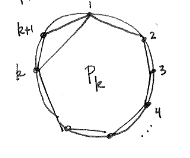
\includegraphics[width=100]{Midterm two/screenshot_2017-03-03_16-17-22.png}
\end{center} Imagine, any number of
edges \(k\), where the first edge is named 1. One could simply add another
\(k+1\) edge to the list.

\item \uline{Example}: Prove that any \(2^n\times2^n\) grid of squares with any one
square removed can be tiled with \emph{L}-shaped tiles.

\begin{figure}[htbp]
\centering
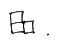
\includegraphics[width=50]{Midterm two/screenshot_2017-03-03_15-48-14.png}
\Leftarrow\textit{L-shaped tiles}
\end{figure} Removing any box
results in the remaining boxes being an \emph{L}-shaped tile.

\begin{figure}[htbp]
\centering
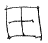
\includegraphics[width=50]{Midterm two/screenshot_2017-03-03_16-00-29.png}
\Leftarrow\textit{box}
\end{figure} 

\begin{center}
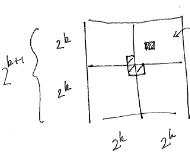
\includegraphics[width=125]{Midterm two/screenshot_2017-03-03_16-01-43.png}
\end{center} A large block can be
covered by \emph{L}-shapes by hypothesis. What about other 3 blocks?

Inductive hypothesis doesn't apply to grid \(2^k\times2^k\) \uline{without}
removing a square. Meaning without removing one atomic box.

\uline{Solution}: consider removing a single \emph{L} instead, taking away a box from
three quadrants. It is an equivalent procedure.
\end{itemize}

\section{Midterm three}
\label{sec:org40a7fff}
\subsection{Boundaries}
\label{sec:org266f16c}
\begin{definition}[Interior Point and Boundary Point]
  Let $S$ be a subset of $\Real$. A point $x$ in $\Real$ is an
  \textit{\textbf{interior point}} of $S$ if there exists a neighborhood $N$
  of $x$ such that $N \sube S$. If for every neighborhood $N$ of $x$, $N \cap
  S \ne \varnothing$ and $N \cap (\Real \setminus S) \ne \varnothing$, then $x$ is called a
  \textit{\textbf{boundary point}} of $S$. The set of all interior points of
  $S$ is denoted by int $S$, and the set of all boundary points of $S$ is
  denoted by $\bd{S}$.
\end{definition}

\begin{definition}[Neighborhood]
  Let $x\in\Real$ and let $\varepsilon>0$. A \textit{\textbf{neightborhood}}
  of $x$ (or an \textit{\textbf{$\varepsilon$-neightborhood}} of $x$) is a
  set of the form $N(x; \varepsilon) = \{ y \in \Real : \abs{x - y} < \varepsilon \}$.
  \begin{remark}
    The professor uses the notation: $$N_\varepsilon(x) = \{ y \in \Real :
    \abs{x - y} < \varepsilon \},$$ which is probably nicer.
  \end{remark}
\end{definition}

\begin{definition}[Deleted Neighborhood]
  Let $x \in \Real$ and let $\varepsilon > 0$. A \textit{\textbf{deleted neighborhood}} of
  $x$ is a set of  the form $N^*(x; \varepsilon)=\{ y \in \Real : 0 <  \abs{x - y} < \varepsilon\}$.
  Clearly, $N^*(x; \varepsilon) = N(x; \varepsilon) \setminus \{ x \}$
  \begin{remark}
    The professor uses the notation: $$N_\varepsilon^*(x) = \{  y \in \Real : 0 < \abs{x -
    y} < \varepsilon\},$$ which is probably nicer.
  \end{remark}
\end{definition}

\begin{definition}[Open and Closed Sets]
  Let   $S  \sube   \Real$.  If   $\bd{S}  \sube   S$,  then   $S$  is   said  to   be
  \textit{\textbf{closed}}. If  $\bd{S} \sube \Real \setminus  S$, then $S$ is  said to be
  \textit{\textbf{open}}.
\end{definition}

\begin{theorem}
  \begin{itemize}
  \item A set $S$ is open $\iff$ $S = \interior S$. Equivalently, $S$ is open $\iff$
    every point in $S$ is an interior point of $S$.

  \item A set $S$ is closed $\iff$ its complement $\Real \setminus S$ is open.
  \item The union of any collection of open sets is an open set.
  \item The intersection of any finite collection of open sets is an open set.
  \end{enumerate}
\end{theorem}

\subsection{Topology of the Real Numbers}
\label{sec:org67b264d}
Every bounded sequence has a convergent subsequence.
\begin{itemize}
\item If \(\{s_n\}\) bounded, then
\begin{enumerate}
\item for every \(\varepsilon\), \(\exists N \in \Natural \ni s_n < m + \varepsilon\) when \(n \ge N\). (Else there
are infinitely  many \(s_n \ge  m + \varepsilon\), so  there can't be  a lim
sup.)
\item for every \(\varepsilon > 0\), \(\forall i \in \Natural, \exists k>i\) with \(s_k > m - \varepsilon\).
(There are infinitely many  \(s_k \in (m-\varepsilon, m+\varepsilon)\), else
\(m-\varepsilon\) is upper bound for all limits of subsequences.)
\end{enumerate}
\end{itemize}

\begin{definition}[Accumulation Points]
  Let $S$ be a subset of $\Real$. A point $x$ in $\Real$ is an
  \textbf{accumulation point} of $S$ if every deleted neighborhood of $x$
  contains a point of $S$. That is, for every $\varepsilon > 0$, $N^{*}(x,\varepsilon) \cup S \ne
  \varnothing$. The set of all accumulation points of $S$ is denoted by
  $S\pr$. If $x\in S$ and $x\notin S\pr$, then $x$ is called an \textbf{isolated
  point} of $S$.
\end{definition}

\begin{definition}[Closure]
  Let $S \sube \Real$. Then the closure of $S$, denoted $\text{cl } S$, is
  defined by $$\text{cl } S = S \cup S\pr,$$ where $S\pr$ is the set of all
  accumulation points of $S$.

  Also, $$\text{cl } S = S \cup \text{bd } S.$$
\end{definition}

\subsection{Compact Sets}
\label{sec:org82b3fa3}
\begin{definition}[Compact, Open Cover, and Subcover]
  A set $S$ is said to be \textit{\textbf{compact}} if whenever it is
  contained in the union of a family $\F$ of open sets, it is contained in
  the union of some finite number of the sets in $\F$. If $\F$ is a family of
  open sets whose union contains $S$, then $\F$ is called an
  \textit{\textbf{open cover}} of $S$. If $\G \sube \F$ and $\G$ is also an open
  cover of $S$, then $\G$ is called a \textit{\textbf{subcover}} of $S$.

  \begin{corollary}
      $S$ is compact $\overset{Heine-Borel}{\iff}$ $S$ is closed and bounded
      $\iff$ every infinite subset of S has an accumulation point in $S$.

      $S$ is a nonempty closed bounded subset of $\Real$ $\Rightarrow$ $S$ has a maximum
      and a minimum.
  \end{corollary}
\end{definition}

\begin{definition}[Heine--Borel]
  A subset $S$ of $\Real$ is compact iff $S$ is closed and bounded.
\end{definition}

\begin{definition}[Bolzano--Weierstrass]
  If a bounded subset $S$ of $\Real$ contains infinitely many points, then there
  exists at least one point in $\Real$ that is an accumulation point of $S$.
\end{definition}

\subsection{Sequences}
\label{sec:org69964c4}
\begin{definition}[Sequence]
  A sequence $S$ is a function whose domain is the set $\Natural$ of natural
  numbers. Denoted by its value of $n$ at $s_n$ instead of $S(n)$ or by listing
  its values $(s_1, s_2, s_3, ...)$. $s_n$ is the $n^{th}$ term of the sequence.
\end{definition}

\begin{definition}[Convergence, Divergence, Limit]
  A sequence $(s_n)$ is said to \textbf{\textit{converge}} to the real number
  $s$ provided that
  \begin{center}
    for every $\varepsilon > 0$ there exists a natural number $N$ such that for
    all $n \in \Natural$, $n \ge N$ implies that $\abs{s_n - s} < \varepsilon$.
  \end{center}
  If $(s_n)$ converges to $s$, then $s$ is called the \textbf{\textit{limit}}
  of the sequence $(s_n)$, and we write $\underset{n\rightarrow\infty}{\text{lim}} s_n = s$,
  lim $s_n = s$, or $s_n \rightarrow s$. If a sequence does not converge to a real
  number, it is said to \textbf{\textit{diverge}}.
\end{definition}

\begin{definition}[Subsequence]
Let $(s_n)_{n=1}^\infty$ be a sequence and let $(n_k)_{k=1}^{\infty}$ be any sequence
of natural numbers such that $n_1 < n_2 < ...$. The sequence
$(s_{n_k})_{k=1}^{\infty}$ is called a \textit{\textbf{subsequence}} of
$(s_n)_{n=1}^\infty$.
\end{definition}

\begin{definition}[Limit Superior and Limit Inferior]
  Let $(s_n)$ be a bounded sequence. A \textbf{\textit{subsequential limit}}
  of $(s_n)$ is any real number that is the limit of some subsequence of
  $(s_n)$. If $S$ is the set of all subsequential limits of $(s_n)$, then we
  define the \textbf{\textit{limit superior}} (or \textbf{\textit{upper
  limit}}) of $(s_n)$ to be $$\text{lim sup } s_n = \text{sup } S.$$
  Similarly, we define the \textit{\textbf{limit inferior}} (or
  \textit{\textbf{lower limit}}) of $(s_n)$ to be $$\text{lim inf } s_n =
  \text{inf } S.$$
\end{definition}

\begin{definition}[Bounded Sequence]
  A sequence $(s_n)$ is said to be \textit{\textbf{bounded}} if the range $\{
  s_n : n \in \Natural \}$ is a bounded set, that is, if there exists an $M \ge
  0$ such that $\abs{s_n} \le M$ for all $n \in \Natural$

  Every convergent sequence is bounded.

  If a sequence converges, its limit is unique.

  Every bounded sequence has a convergent subsequence.
\end{definition}

\subsection{Limit Theorem}
\label{sec:orgb063131}
\begin{definition}[Limit Theorems]
  \begin{enumerate}
    \item $\lim{(s_n + t_n)} = s + t$
    \item $\lim{(ks_n)} = ks$ and $\lim{(k + s_n)} = k + s$, for any $k \in
      \Real$
    \item $\lim{(s_n t_n)} = st$
    \item $\lim{(s_n/t_n)} = s/t$, provided that $t_n \ne 0$ for all $n$ and $t
      \ne 0$
  \end{enumerate}
\end{definition}

\begin{definition}[Lesser Convergence]
  Suppose that $(s_n)$ and $(t_n)$ are convergent sequences with $\lim{s_n} =
  s$, and $\lim{t_n} = t$. If $s_n \le t_n$ for all $n \in \Natural$, then $s
  \le t$.
\end{definition}

\begin{corollary}
  If $(t_n)$ converges to $t$ and $t_n \ge 0$ for all $n \in \Natural$, then $t
  \ge 0$.
\end{corollary}

\begin{definition}[Ratio Convergence]
  Suppose that $(s_n)$ is a sequence of positive terms and that the sequence of
  rations $(s_{n+1} / s_n)$ converges to $L$. If $L < 1$, then $\lim{s_n} = 0$
\end{definition}

\begin{definition}[Divergence]
  A sequence $(s_n)$ is said to \textit{\textbf{diverge to}} $+\infty$, and we
  write $\lim{s_n} = +\infty$ provided that
  \begin{center}
    for every $M \in \Real$ there exists a natural number $N$ such that $n \ge
    N$ implies that $s_n > M$.
  \end{center}

  A sequence $(s_n)$ is said to \textit{\textbf{diverge to}} $-\infty$, and we
  write $\lim{s_n} = +\infty$ provided that
  \begin{center}
    for every $M \in \Real$ there exists a natural number $N$ such that $n \ge
    N$ implies that $s_n < M$.
  \end{center}
\end{definition}

\begin{definition}[Greater Divergence]
  Suppose that $(s_n)$ and $(t_n)$ are sequences such that $s_n \le t_n$ for all
  $n \in \Natural$.
  \begin{enumerate}
    \item If $\lim{s_n} = +\infty$, then $\lim{t_n} = +\infty$.
    \item If $\lim{t_n} = -\infty$, then $\lim{s_n} = -\infty$.
  \end{enumerate}
\end{definition}

\begin{definition}[Inverse of Divergence]
Let $(s_n)$ be a sequence of positive numbers. Then $\lim{s_n} = +\infty$ $\iff$
$\lim{(1/s_n)} = 0$.
\end{definition}

\subsection{Monotone Sequences and Cauchy Sequences}
\label{sec:org6f63b9d}
\begin{definition}[Monotone Sequences]
  A sequence $(s_n)$ of real numbers is \textit{\textbf{increasing}} if $s_n \le
  s_{s_n+1}$ for all $n \in \Natural$ and is \textit{\textbf{decreasing}} if
  $s_n \ge s_{n+1}$ for all $n \in \Natural$. A sequence is
  \textbf{\textit{monotone}} if it is increasing or decreasing.
\end{definition}

\begin{definition}[Monotone Convergence Theorem]
  A monotone sequence is convergent $\iff$ it is bounded.
\end{definition}

\begin{definition}[Cauchy Sequence]
If, for every $\varepsilon>0$, there exists $N \in \Natural$ such that if $m,n \ge N$ then
$\abs{s_n - s_m} < \varepsilon$.

Every convergent sequence is \textit{\textbf{Cauchy}}.

If $(s_n)$ is a \textit{\textbf{Cauchy}} sequence, then $(s_n)$ converges.
\end{definition}

\begin{proof}
   Given any $\varepsilon > 0$, choose $N$ such that $\abs{s_n - s} < \frac{\epsilon}{2}$ if
  $n \ge N$ (which is possible to do since $s_n \rightarrow s$). Then $\abs{s_n - s_m} =
  \abs{s_n - s + s - s_m}$ because adding and subtracting by the limit is the
  same as doing nothing, and, by the triangle inequality, $\abs{s_n - s + s -
  s_m} \le \abs{s_n - s} + \abs{s_m - s} < \frac{\varepsilon}{2} + \frac{\varepsilon}{2}$.
\end{proof}

\section{Final}
\label{sec:org0c692d8}
\subsection{Limits of Functions}
\label{sec:orgaa0a514}
\begin{definition}[Limit of $f$ at $c$]
  Let $f : D \rightarrow \Real$ and let $c$  be an accumulation point of $D$. We
  say that a real number $L$ is a limit of $f$ at $c$, if
  \begin{center}
    for each $\varepsilon > 0$ there exists a $\delta > 0$ such that $\abs{f(x)
      - L)} < \varepsilon$ whenever $x \in D$ and $0 < \abs{x - c} < \delta$.
  \end{center}
\end{definition}

\begin{theorem}
  Let $f : D \rightarrow \Real$ and let $c$  be an accumulation point of $D$.
  Then $\lim_{x \rightarrow c} f(x) = L$ $\iff$ for each neighborhood $V$ of $L$
  there exists a deleted neighborhood $U$ of $c$ such that $f(U \cap D) \sube V$.
\end{theorem}

\begin{theorem}
Let $f : D \rightarrow \Real$ and let $c$ be an accumulation point of $D$. Then
$\lim_{x \rightarrow c} f(x) = L$ $\iff$ for every sequence $(s_n)$ in $D$ that
converges to $c$ with $s_n \ne c$ for all $n$, the sequences $(f(s_n))$
converges to $L$.
\end{theorem}

\begin{theorem}
  Let $f : D \rightarrow \Real$ and let $c$ be an accumulation point of $D$.
  Then the following are equivalent:
  \begin{enumerate}
  \item $f$ does not have a limit at $c$.
  \item There exists a sequence $(s_n)$ in $D$ with each $s_n \ne c$ such that
    $(s_n)$ converges to $c$, but $(f(s_n))$ is not convergent in $\Real$.
  \end{enumerate}
\end{theorem}

\subsection{Continuity}
\label{sec:orgece7594}
\begin{definition}[Continuous]
  Let $f  : D \rightarrow \Real$  and let $c$ be  an accumulation point of  $D$. We say
  that $f$ is continuous at $c$, if
  \begin{center}
    for each $\varepsilon > 0$  there exists a $\delta > 0$ such that  $\abs{f(x) - L)} < \varepsilon$
    whenever $x \in D$ and $\abs{x - c} < \delta$.
  \end{center}
  If $f$ is continuous at each point of a subset $S$ of $D$, then $f$ is said
  to be \textbf{continuous on $S$}. If $f$ is continuous on its domain $D$,
  then $f$ is said to be a \textbf{continuous function}.
\end{definition}

\begin{theorem}
  Let $f : D \rightarrow \Real$ and let $c \in D$. Then the following three
  conditions are equivalent:
  \begin{enumerate}
  \item $f$ is continuous at $c$.
  \item If $(x_n)$ is any sequence in $D$ such that $(x_n)$ converges to $c$,
    then $\lim_{n \rightarrow \infty} f(x) = f(c)$.
  \item For every neighborhood $V$ of $f(c)$ there exists a neighborhood $U$ of
    $c$ such that $f(U \cap D) \sube V$.
  \item If $c$ is an accumulation point of $D$, then $f$ has a limit at $c$ and
    $\lim_{x \rightarrow c} f(x) = f(c)$.
  \end{enumerate}
\end{theorem}

\begin{theorem}
  Let $f : D \rightarrow \Real$ and let $c \in D$. Then $f$ is discontinuous at
  $c$ $\iff$ there exists a sequence $(x_n)$ in $D$ such that $(x_n)$ converges
  to $c$ but the sequence $(f(x_n))$ does not converge to $f(c)$.
\end{theorem}

\begin{theorem}
  Let $f : D \rightarrow \Real$ and let $c \in D$. Suppose that $f$ and $g$ are
  continuous at $c$. Then
  \begin{enumerate}
  \item $f + g$ and $fg$ are continuous at $c$, and
  \item $f / g$ is continuous at $c$ if $g(c) \ne 0$
  \end{enumerate}
\end{theorem}

\begin{theorem}
  Let $f : D \rightarrow \Real$ and $g : E \rightarrow \Real$ be functions such
  that $f(D) \sube E$. If $f$ is continuous at a point $c \in D$ and $g$ is
  continuous at $f(c)$, then the composition $g \circ f : D \rightarrow \Real$
  is continuous at $c$.
\end{theorem}

\begin{theorem}
  A function $f : D \rightarrow \Real$ is continuous on $D$ $\iff$ for every
  open set $G \sube \Real$ there exists an open set $H \sube \Real$ such that $H \cap
  D = f^{-1}(G)$.
\end{theorem}

\begin{corollary}
  A function $f: \Real \rightarrow \Real$ is continuous $\iff$ $f^{-1}(G)$ is
  open in $\Real$ whenever $G$ is open in $\Real$.
\end{corollary}

\subsection{Properties of Continuous Functions}
\label{sec:org92d4deb}
\begin{definition}[Bounded]
  A function $f: D \rightarrow \Real$ is said to be bounded if its range $f(D)$
  is a bounded subset of $\Real$. That is, $f$ is bounded if there exists $M \in
  \Real$ such that $\abs{f(x)} \le M$ for all $x \in D$
\end{definition}

\begin{theorem}
  Let $D$ be a compact subset of $\Real$ and suppose that $f : D \rightarrow
  \Real$ is continuous. Then $f(D)$ is compact.
\end{theorem}

\begin{corollary}
  Let $D$ be a compact subset of $\Real$ and suppose that $f : D \rightarrow
  \Real$ is continuous. Then $f$ assumes minimum and maximum values on $D$. That
  is, there exist points $x_1$ and $x_2$ in $D$ such that $f(x_1) \le f(x) \le
  f(x_2)$ for all $x \in D$.
\end{corollary}

\begin{lemma}
  Let $f : [a,b] \rightarrow \Real$ be continuous and suppose that $f(a) < 0 <
  f(b)$. Then there exists a point $c$ in $(a,b)$ such that $f(c) = 0$.
\end{lemma}

\begin{definition}[Intermediate Value Theorem]
  Suppose that $f : [a,b] \rightarrow \Real$ is continuous. Then $f$ has the
  intermediate value property on $[a,b]$. That is, if $k$ is any value between
  $f(a)$ and $f(b)$ [\textit{i.e.}, $f(a) < k < f(b)$ or $f(b) < k < f(a)$],
  then there exists $c \in (a,b)$ such that $f(c) = k$.
\end{definition}

\begin{theorem}
  Let $I$ be a compact interval and suppose that $f : I \rightarrow \Real$ is a continuous
  function. Then the set $f(I)$ is a compact interval.
\end{theorem}

\subsection{Uniform Continuity}
\label{sec:org6d1f5e5}
\begin{definition}[Uniform Continuity]
  Let $f : D \rightarrow \Real$. We say that $f$ is \textbf{uniformly continuous} on
  $D$ if
  \begin{center}
    for every $\varepsilon > 0$ there exists a $\delta > 0$ such that $\abs{f(x)
      - f(y)} < \varepsilon$ whenever $\abs{x - y} < \delta$ and $x,y \in D$.
  \end{center}
  A function is continuous at a point, but uniform continuity is a property of a
  that applies to a function \textit{on a set}. We never speak of a function
  being uniformly continuous at a point.
\end{definition}

\subsection{Differentiation}
\label{sec:org97b2d8e}
\begin{definition}[Derivative]
  Let $f$ be a real-valued function defined on an interval $I$ containing the
  point $c$. (We  allow the possibility that  $c$ is an endpoint  of $I$.) We
  say that $f$ is  differentiable at $c$ (or has a derivative  at $c$) if the
  limit $$\underset{x  \rightarrow c}{\lim} \frac{f(x) -  f(c)}{x - c}$$ exists  and is
  finite.  We denote  the  derivative of  $f$  at $c$  by  $f\pr(c)$ so  that
  $$f\pr(c) = \underset{x \rightarrow c}{\lim} \frac{f(x) - f(c)}{x - c}$$ whenever the
  limit exists and  is finite. If the function $f$  is differentiable at each
  point of the set $S \sube I$, then $f$ is said to be differentiable on $S$, and
  the function $f\pr : S \rightarrow \Real$ is called the derivative of $f$ on $S$.
\end{definition}

\begin{theorem}
  Let $I$ be an  interval containing the point $c$ and suppose that  $f : I \rightarrow
  \Real$. Then $f$ is differentiable at $c$ $\iff$ for every sequence $(x_n)$
  in $I$  that converges  to $c$  with $x_n \ne  c$ for  all $n$,  the sequence
  $$\left( \frac{f(x_n) - f(c)}{x_n - c} \right)$$ converges. Furthermore, if
  $f$ is  differentiable at $c$,  then the  sequence of quotients  above will
  converge to $f\pr(c)$.
\end{theorem}

\begin{theorem}
  If $f : I \rightarrow \Real$ is differentiable at a point $c \in I$, then $f$ is
  continuous at $c$.
\end{theorem}

\begin{theorem}
  Suppose that $f : I \rightarrow \Real$ and $g : I \rightarrow \Real$ are differentiable at $c \in
  I$. Then
  \begin{enumerate}
  \item If $k \in \Real$, then the function $kf$ is differentiable at $c$
    and $$(kf)\pr(c) = k \cdot f\pr(c).$$
  \item The function $f + g$ is differentiable at $c$ and $$(f + g)\pr(c) =
    f\pr(c) + g\pr(c)$$
  \item (Product Rule) The function $fg$ is differentiable at $c$
    and $$(fg)\pr(c) = f(c)g\pr(c) + g(c)f\pr(c)$$
  \item (Quotient Rule) If $g(c) \ne 0$, then the function $f / g$ is
    differentiable at $c$ and $$\left( \frac{f}{g} \right)\pr (c) =
    \frac{g(c)f\pr(c) - f(c)g\pr(c)}{[g(c)]^2}$$
  \end{enumerate}
\end{theorem}

\begin{theorem}
(Chain Rule) Let $I$ and $J$ be intervals in $\Real$, let $f : I \rightarrow \Real$ and
$g : J \rightarrow \Real$, where $f(I) \sube J$, and let $c \in I$. If $f$ is differentiable
at $c$ and $g$ is differentiable at $f(c)$, then the composite function $g \circ f$ is
differentiable at $c$ and $$(g \circ f)\pr(c) = g\pr(f(c)) \cdot f\pr(c)$$
\end{theorem}

\subsection{The Mean Value Theorem}
\label{sec:org586e70c}
\begin{theorem}
  If $f$ is differentiable on an open interval $(a,b)$ and if $f$ assumes its
  maximum or minimum at a point $c \in (a,b)$, then $f\pr(c) = 0$.
\end{theorem}

\begin{theorem}
  (Rolle's Theorem) Let $f$ be a continuous function on $[a,b]$ that is
  differentiable on $(a,b)$ and such that $f(a) = f(b)$. Then there exists at
  least one point $c$ in $(a,b)$ such that $f\pr(c) = 0$.
\end{theorem}

\begin{theorem}
  (Mean Value Theorem) Let $f$ be a continuous function on $[a,b]$ that is
  differentiable on $(a,b)$. Then there exists at least one point $c \in (a,b)$
  such that $$f\pr(c) = \frac{f(b) - f(a)}{b - a}.$$
\end{theorem}

\begin{theorem}
  Let $f$ be continuous on $[a,b]$ and differentiable on $(a,b)$. If $f\pr(x)
  = 0$ for all $x \in (a,b)$, then $f$ is constant on $[a,b]$.
\end{theorem}

\begin{corollary}
  Let $f$ and $g$ be continuous an $[a,b]$ and differentiable on $(a,b)$.
  Suppose that $f\pr(x) = g\pr(x)$ for all $x \in (a,b)$. Then there exists a
  constant $C$ such that $f = g + C$ on $[a,b]$.
\end{corollary}

\begin{theorem}
  Let f be differentiable on an interval $I$. Then 
  \begin{enumerate}
  \item if $f\pr(x) > 0$ for all $x \in I$, then $f$ is strictly increasing on
    $I$, and
  \item if $f\pr(x) < 0$ for all $x \in I$, then $f$ is strictly decreasing on
    $I$.
  \end{enumerate}
\end{theorem}

\begin{theorem}
  (Intermediate Value Theorem for Derivatives) Let $f$ be differentiable on
  $[a,b]$ and suppose that $k$ is a number between $f\pr(a)$ and $f\pr(b)$.
  Then there exists a point $c \in (a,b)$ such that $f\pr(c) = k$.
\end{theorem}

\begin{theorem}
  (Inverse Function Theorem) Let $f$ be differentiable on an interval $I$ and
  $f\pr(x) \ne 0$ for all $x \in I$. Then $f$ is injective, $f^{-1}$ is
  differentiable on $f(I)$, and $$(f^{-1})\pr(y) = \frac{1}{f\pr(x)},$$ where
  $y = f(x)$
\end{theorem}

\subsection{Taylor's Theorem}
\label{sec:orgaa04587}
\begin{theorem}
  (Taylor's Theorem) Let $f$ and its first $n$ derivatives be continuous on
  $[a,b]$ and differentiable on $(a,b)$, and let $x_0 \in [a,b]$. Then for each
  $x \in [a,b]$ with $x \ne x_0$ there exists a point $c$ between $x$ and $x_0$
  such that
  \begin{dmath*}
    f(x) = f(x_0) + f\pr(x)(x - x_0) + \frac{f\pr\pr(x_0)}{2}(x - x_0)^2 + ... \\
    + \frac{f^{(n)}(x_0)}{n!}(x - x_0)^n + \frac{f^{(n+1)}(c)}{(n+1)!}(x - x_0)^{n+1}.
  \end{dmath*}
\end{theorem}

\subsection{Integration}
\label{sec:orgc4ae2d2}
\begin{definition}[Partition]
  Let $[a,b]$ be an interval in $\Real$. A \textbf{partition} $P$ of $[a,b]$ is
  a finite set of points $\{ x_0, x_1, ..., x_n \}$ such that $$a = x_0 < x_1 <
  ... < x_n = b.$$ If $P$ and $Q$ are two partitions of $[a,b]$ with $P \sube
  Q$, then $Q$ is called a \textbf{refinement} of $P$.
\end{definition}

\begin{definition}[Upper and Lower Sum]
  Suppose that $f$ is a bounded function defined on $[a,b]$ and that $P = \{
  x_0, ..., x_n \}$ is a partition of $[a,b]$. For each $i = 1, ..., n$ we
  let $$M_i(f) = \sup \{ f(x) : x \in [x_{i-1}, x_i] \}$$ and $$m_i(f) = \inf \{
  f(x) : x \in [x_{i-1}, x_i] \}.$$ When only one function is under
  consideration, we may abbreviate thes to $M_i$ and $m_i$, respectively.
  Letting $\Delta x_i = x_i - x_{i-1} (i = 1, ..., n)$, we define the
  \textbf{upper sum} of $f$ with respect to $P$ to be $$U(f,P) =
  \sum_{i=1}^{n} M_i \Delta x_i,$$ and the \textbf{lower sum} of $f$ with respect
  to $P$ to be $$L(f,P) = \sum_{i=1}^{n} m_i \Delta x_i.$$

  Since we are assuming that $f$ is a bounded function on $[a,b]$, there
  exist numbers $m$ and $M$ such that $m \le f(x) \le M$ for all $x \in [a,b]$.
  Thus for any partition P of [a,b] we have $$m(b - a) \le L(f, P) \le U(f, P) \le
  M(b - a).$$ This implies that the uuper and lower sums for $f$ form a
  bounded set, and it guarantees the existence of the following upper and
  lower integrals of $f$.

  \begin{remark}[History]
  (Sometimes $U(f,P)$ and $L(f,P)$ are called the upper and lower Darboux
  sums in honor of Gaston Darboux (1842--1917), who first developed this
  approach to the Riemann integral.)
  \end{remark}
\end{definition}

\begin{definition}[Upper and Lower Integral]
  Let $f$ be a bounded function defined on $[a,b]$. Then $$U(f) = \inf \{ U(f,
  P) : P \text{ is a partition of } [a,b] \}$$ is called the \textbf{upper integral}
  of $f$ on $[a,b]$. Similarly, $$L(f) = \sub \{ L(f, P) : P \text{ is a
  partition of } [a,b] \}$$ is called the \textbf{lower integrals} of $f$ on
  $[a,b]$, and we denote their common value by $\int_a^b f$ or by $\int_a^b f(x)
  dx$. That is, if L(f) = U(f), then $$\int_a^b f = \int_a^b f(x) dx = L(f) =
  U(f)$$ is the \textbf{Riemann integral} of $f$ on $[a,b]$.

  When convenient, refer to the function $f$ as being \textbf{integrable} on
  $[a,b]$ and call $\int_a^b f$ the \textbf{integral} of $f$ on $[a,b]$.
\end{definition}

\begin{theorem}
  Let $f$ be a bounded function on $[a,b]$. If $P$ and $Q$ are partitions of
  $[a,b]$ and $Q$ is a refinement of $P$, then $$L(f, P) \le L(f, Q) \le U(f, Q) \le
  U(f, P).$$
\end{theorem}

\begin{theorem}
  Let $f$ be a bounded function on $[a,b]$. Then $L(f) \le U(f)$.
\end{theorem}

\begin{theorem}
  Let $f$ be a bounded function on $[a,b]$. Then $f$ is integrable $\iff$ for
  each $\varepsilon > 0$ there exists a partition $P$ of $[a,b]$ such that $$U(f, P) -
  L(f, P) < \varepsilon.$$
\end{theorem}

\begin{theorem}
(The Fundamental Theorem of Calculus I) Let $f$ be integrable on $[a,b]$. For
each $x \in [a,b]$, let $$F(x) = \int_a^x f(t) dt.$$ Then $F$ is uniformly
continuous on $[a,b]$. Furthermore, if $f$ is continuous on $c \in [a,b]$, then
$F$ is differentiable at $c$ and $F\pr(c) = f(c)$.
\end{theorem}

\subsection{Infinite Series}
\label{sec:org0399c08}
\end{document}